\section{実装}

\begin{figure}[tb]
  \centering
  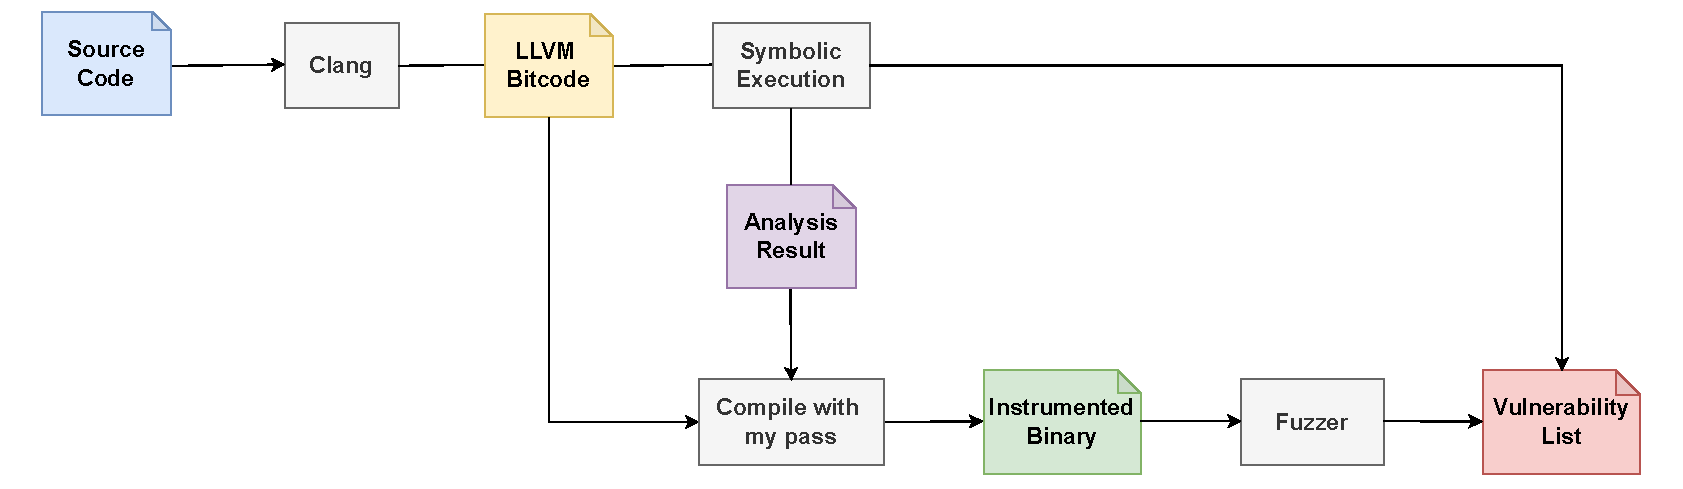
\includegraphics[width=\linewidth]{img/overall.drawio.pdf}
  \caption{提案手法の全体像}\label{fig:overall}
\end{figure}

提案手法の全体像を図\ref{fig:overall}に示す。提案手法では、記号実行をKLEESpectreを元に、ファザーをSpecFuzzを元に実装した。記号実行フェーズでは、LLVM IRを対象にOrderによる制限を加えた記号実行を行い、解析結果をファジングフェーズに提供する。ファジングフェーズでは、LLVM MIRレベルのPassを用いて、分岐予測ミスのシミュレーション用の計装と、記号実行フェーズで得られた解析結果に基づく計装を施したバイナリを生成する。この計装済みのバイナリを、カバレッジ駆動型のファジングツールであるhonggfuzz\cite{Honggfuzz}を使用してファジングを行う。スコアに基づくシードのスケジューリングは、honggfuzzを拡張することで実現している。以降では、提案手法の詳細な実装について詳しく説明する。\par

\subsection{記号実行フェーズ}
\subsubsection{Orderによる分岐予測ミスの制限}
Order値は、ユーザがコマンドラインオプションを通じて設定可能であり、デフォルト値は1に設定されている。記号実行における状態を表現するデータ構造に、現在のネストされた分岐予測ミスの回数を追跡するためのメンバ変数\var{specBranchCount}を追加し、新たな投機的状態がフォークされるたびに、\var{specBranchCount}をインクリメントする。また、投機的な状態をフォークする前に、現在の状態における\var{specBranchCount}が設定されたOrder値を超えていないかを確認する。Order値を超えていない場合は通常通りフォーク処理が行われるが、超えている場合はフォーク処理を行わず、投機的な状態の生成を抑制する。\par

\subsubsection{異常終了した投機的な状態の扱い}
記号実行では、いくつかの要因により投機的な状態が正常に終了しない場合がある。たとえば、ユーザが指定したメモリ使用量の上限やスタック数の上限に達した場合、一部の状態の探索が途中で打ち切られることがある。記号実行フェーズでRemovable Directionを特定する際、このような理由で探索が途中で終了し、ターゲット状態に到達できなかった場合、解析が継続していれば到達可能だったかどうかを判断することができない。そのため、このようなケースではその分岐予測ミスによりターゲット状態に到達する可能性があると保守的に判断し、Removable Directionではないと記録する。逆にRemovable Directionとして記録される可能性があるのは、投機的な状態が正常に終了した場合のみである。正常に終了したと判断されるのは以下のいずれかの場合のみである。\par

\begin{itemize}
  \item 投機ウィンドウの上限に達した場合
  \item 直列化命令に遭遇した場合
  \item プログラムが終了した場合
\end{itemize}

\subsection{ファジングフェーズ}
\subsubsection{分岐予測ミスの抑制を行う計装}
Removable Directionの分岐予測ミスのシミュレーションを抑制するための計装を行うアルゴリズムをAlgorithm\ref{alg:suppress_misspredication}に示す。まず各基本ブロックの終端命令を確認し、それが分岐命令であるかを調べる。分岐命令である場合、記号実行の解析結果\ref{Unnecessary_branch_result}内に該当する分岐命令が存在するかを確認する。この確認は、分岐命令の位置情報(\var{location})が一致するかどうかで行う。Removable Directionであると判断されている場合(\var{truePath}または\var{falsePath}が\var{true}である場合)、該当分岐方向の遷移先となる基本ブロックの先頭に、ランタイム関数\var{force\_rlbk}の呼び出しを挿入する。ランタイム関数\var{force\_rlbk}は、直前の分岐命令が分岐予測ミスされていた場合、シミュレーションを終了させ、即座にロールバックさせる。この計装により、Removable Directionの分岐予測ミスが発生した場合でも、即座にシミュレーションを終了させることができる。\par

\begin{algorithm}
\caption{Removable Directionの分岐予測ミスの抑制のための計装を行うアルゴリズム}
\label{alg:suppress_misspredication}
\begin{algorithmic}[H]

\State \textbf{Input:}
\State \hspace{1em} CFG: Control Flow Graph of the target program at LLVM MIR level
\State \hspace{1em} Result: Analysis results containing unnecessary branch misprediction information

\Function{Suppress\_Misprediction}{Result, CFG}
    \ForAll{BasicBlock \text{B} in CFG}
        \State $\text{Terminator} \gets \text{B.getTerminator()}$
        \If{$\text{Terminator.isConditionalBranch()}$}
            \State $\text{Location} \gets \text{Terminator.getLocation()}$
            \State $\text{BranchInfo} \gets \text{findBranchInfo}(\text{Result}, \text{Location})$

            \If{$\text{BranchInfo}$ exists}
                \If{$\text{BranchInfo.truePath} = \text{true}$}
                    \State $\text{TrueBlock} \gets \text{Terminator.getTakenSuccessor()}$
                    \State \text{addCallRuntimeFunction}($\text{TrueBlock}$, ``force\_rlbk'')
                \EndIf

                \If{$\text{BranchInfo.falsePath} = \text{true}$}
                    \State $\text{FalseBlock} \gets \text{Terminator.getNotTakenSuccessor()}$
                    \State \text{addCallRuntimeFunction}($\text{FalseBlock}$, ``force\_rlbk'')
                \EndIf
            \EndIf
        \EndIf
    \EndFor
\EndFunction

\end{algorithmic}
\end{algorithm}


\subsubsection{スコア計算のための計装}
スコア計算を行うために、テストケースがどの分岐方向を通過したかを記録するための計装を行う。まず、Algorithm\ref{alg:suppress_misspredication}と同様に、対象プログラム内の分岐命令を特定し、記号実行の解析結果\ref{Execution_Trace}内に該当する分岐命令が存在するかを確認する。該当する分岐命令における各分岐方向がTarget Directionであると判断されている場合は(\var{truePath},\var{falsePath},\var{trueSpPath},\var{falseSpPath}のいずれかが1の場合)、その分岐方向を一意に識別するためのインデックスを割り当てる。この時、投機的な分岐方向にも一意のインデックスが割り当てられる。そして、インデックスが割り当てられた分岐方向の遷移先となる基本ブロックの先頭に、ランタイム関数\var{record\_direction}の呼び出しを挿入する。このランタイム関数は分岐方向を識別するインデックスを引数として受け取り、そのインデックスに対応するビットマップ上の位置にビットを立てる。つまり、テストケースが通過したTarget Directionの種類をビットマップを用いて記録する。最終的に、テストケースが通過したTarget Directionの種類数をビットマップから取得し、式\ref{equ:Scoring}に基づきスコアを計算する。\par

\subsubsection{投機ウィンドウの設定}
KLEESpectreとSpecFuzzの違いの一つに、投機実行のシミュレーション中における命令数のカウントの基準が挙げられる。KLEESpectreは解析対象がLLVM IRであるため、LLVM IRレベルの命令数をカウントし、投機ウィンドウの上限に達しているかをチェックする。一方で、SpecFuzzはLLVM MIRレベルの命令数をカウントするコードを計装し、実行時に投機ウィンドウの上限を確認する。この違いにより、単純に2つのツールを併用して同じ投機ウィンドウの上限を設定しても、カウントされる命令レベルが異なるため、投機実行のシミュレーション終了のタイミングにずれが生じ、検出されるGadgetに差が生じる可能性がある。そこで、SpecFuzzの命令数のカウントをLLVM IRレベルで行うように修正し、KLEESpectreと基準を統一した。\par
LLVM IRレベルのパスを用いて、解析対象のコードに実行時のLLVM IRレベルでの命令数をカウントするコードを計装する。シミュレーション中に実行された命令数はグローバル変数\var{instruction\_counter}で管理される。具体的には、各基本ブロックの先頭に、その基本ブロックに含まれるデバッグ命令を除いた命令数を\var{instruction\_counter}に加算するコードを挿入する。シミュレーションが開始されると、\var{instruction\_counter}は0に初期化され、その後、各基本ブロックの先頭で命令数がインクリメントされる。そして、\var{instruction\_counter}の値が投機ウィンドウの上限に達しているかは、各基本ブロックの終端でチェックされる。このチェックに基づいて、シミュレーションを継続するか否かが判断される。

